\section{Artificial example} \label{sec:example}
Within this section, we show how a rather trivial stochastic model of a reading experiment can be implemented using StochBB's Python interface.

The model describes the fixation duration $R$ as a simple chain of a lexical $L$, semantic $S$ and occulomotor $M$ stage. Each stage is represented by a Gamma distributed random variable, that is
\begin{align*}
 L &\sim \Gamma(5\,f+5, 10)\\
 S &\sim \Gamma(10\,p+5, 20)\\
 M &\sim \Gamma(10, 30)\\
 \Rightarrow R &= L+S+M\,,
\end{align*} 
where $f$ is the words log-frequency and $p$ its predictability. In a reading experiment, participants usually do not read a single word with a fixed frequency and predictability but rather read several words with different frequencies and predictabilities. Hence it is necessary to model the predictabilities and frequencies as random variables too, for example
\begin{align*}
 f &\sim U[0,4]\\
 p &\sim U[0,1]\,.
\end{align*}
With this, the lexical ($L$) and semantic ($S$) stages are not Gamma distributed anymore but compound-Gamma distributed. 

The following code shows how this simple model of a reading experiment is implemented using the Python API of StochBB.

\begin{lstlisting}[language=Python]
from numpy import *
import stochbb

# Corpus model:
#  Log word frequency (per mililon), is uniform distr. on the interval [0,4]
f = stochbb.uniform(0,4)
#  Predictability of word is unif. distributed on the interval [0,1]
p = stochbb.uniform(0,1)

# Experimental model:
#  "lexical" stage is gamma distributed with k=5*f+5, theta=10
L = stochbb.gamma(5*f + 5, 10)
#  "semantic" stage is gamma distributed with k=10*p+5, theta=20
S = stochbb.gamma(10*p + 5, 20)
#  "motor" stage is gamma distributed with k=10, theta=30
M = stochbb.gamma(10, 30)
#  "response latency" is simply R = L + S + M
R = L + S + M

# Evaluate marginal densities on interval [0,1200] ms
Tmin, Tmax, N = 0, 1200, 1000
t = linspace(Tmin, Tmax, N); dt = float(Tmax-Tmin)/N
pL = empty(N,); L.density().eval(Tmin, Tmax, pL)
pS = empty(N,); S.density().eval(Tmin, Tmax, pS)
pM = empty(N,); M.density().eval(Tmin, Tmax, pM)
pR = empty(N,); cProfile.run("R.density().eval(Tmin, Tmax, pR)")

# Sample 10k samples from system
sam = stochbb.ExactSampler([L,S,M,R])
X = empty((100000, 4))
sam.sample(X)
\end{lstlisting}

Figure \ref{fig:example} shows the results of the script. The histogram of the samples are in a good agreement with the PDFs obtained numerically. 

\begin{figure}[!ht]
 \centering
 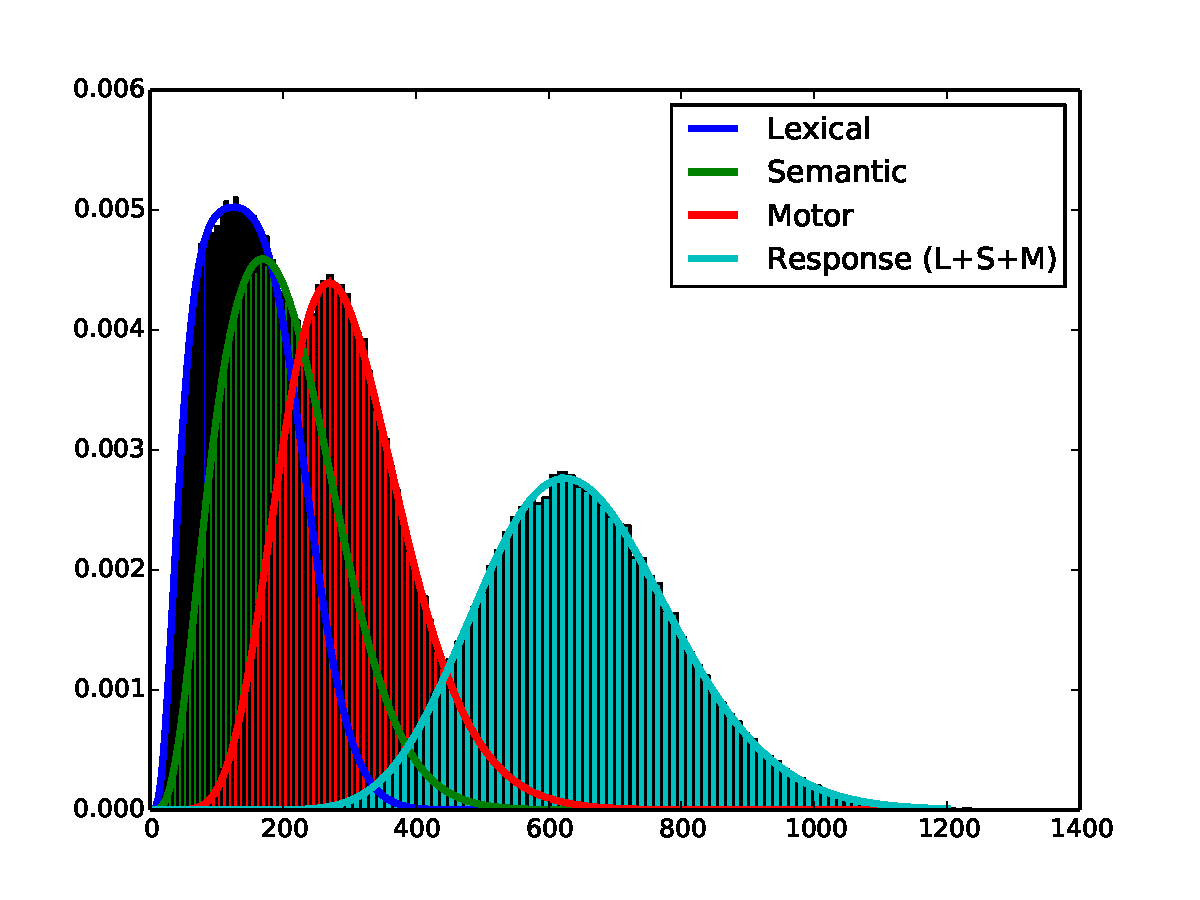
\includegraphics[width=0.6\textwidth]{fig/example.pdf}
 \caption{Shows the histogram of the samples (boxes) and the numerically obtained densities (lines).} \label{fig:example}
\end{figure}